\documentclass[onecolumn, draftclsnofoot,10pt, compsoc]{IEEEtran}
\usepackage{graphicx}
\usepackage{setspace}
\usepackage{comment}
\usepackage{bigstrut}
\usepackage{geometry}
\usepackage{supertabular}
\usepackage{tabu}
\usepackage{hyperref}
\usepackage{url}
\hypersetup{
  colorlinks=true, linkcolor=blue, citecolor=blue, filecolor=blue, urlcolor=blue}
\geometry{textheight=9.5in, textwidth=7in}

\usepackage{color}
\definecolor{editorGray}{rgb}{0.95, 0.95, 0.95}
\definecolor{editorOcher}{rgb}{1, 0.5, 0} % #FF7F00 -> rgb(239, 169, 0)
\definecolor{editorGreen}{rgb}{0, 0.67, 0} % #007C00 -> rgb(0, 124, 0)

\usepackage{listings}
\lstdefinelanguage{JavaScript}{
  morekeywords={typeof, new, true, false, catch, function, return, null, catch, switch,
  var, if, in, while, do, else, case, break, addChapter, await},
  morecomment=[s]{/*}{*/},
  morecomment=[l]//,
  morestring=[b]",
  morestring=[b]'
}

\lstset{%
    % Basic design
    backgroundcolor=\color{editorGray},
    basicstyle={\small\ttfamily},
    frame=l,
    % Line numbers
    xleftmargin={0.75cm},
    numbers=left,
    stepnumber=5,
    firstnumber=1,
    numberfirstline=true,
    % Code design
    keywordstyle=\color{blue}\bfseries,
    commentstyle=\color{red}\ttfamily,
    ndkeywordstyle=\color{editorOcher}\bfseries,
    stringstyle=\color{editorGreen},
    % Code
    language=JavaScript,
    alsodigit={.:;},
    tabsize=2,
    showtabs=false,
    showspaces=false,
    showstringspaces=true,
    extendedchars=true,
    breaklines=true
}


% 1. Fill in these details
\def \CapstoneTeamName{		Remix}
\def \CapstoneTeamNumber{		61}
\def \GroupMemberOne{			Josh Matteson}
\def \GroupMemberTwo{			Steven Powers}
\def \GroupMemberThree{			Evan Tschuy}
\def \CapstoneProjectName{		Many Voices Platform}
\def \CapstoneSponsorCompany{	Oregon State University}
\def \CapstoneSponsorPerson{		Carlos Jensen}

% 2. Uncomment the appropriate line below so that the document type works
\def \DocType{
        %Problem Statement
				%Requirements Document
				%Technology Review
				%Design Document
				Progress Report
				}

\newcommand{\NameSigPair}[1]{\par
\makebox[2.75in][r]{#1} \hfil 	\makebox[3.25in]{\makebox[2.25in]{\hrulefill} \hfill		\makebox[.75in]{\hrulefill}}
\par\vspace{-12pt} \textit{\tiny\noindent
\makebox[2.75in]{} \hfil		\makebox[3.25in]{\makebox[2.25in][r]{Signature} \hfill	\makebox[.75in][r]{Date}}}}
% 3. If the document is not to be signed, uncomment the RENEWcommand below
\renewcommand{\NameSigPair}[1]{#1}

%%%%%%%%%%%%%%%%%%%%%%%%%%%%%%%%%%%%%%%
\begin{document}
\begin{titlepage}
    \pagenumbering{gobble}
    \begin{singlespace}
    	
\includegraphics[height=4cm]{coe_v_spot1}
        \hfill
        % 4. If you have a logo, use this includegraphics command to put it on the coversheet.
        %\includegraphics[height=4cm]{CompanyLogo}
        \par\vspace{.2in}
        \centering
        \scshape{
            \huge CS Capstone \DocType \par
            {\large\today}\par
            \vspace{.5in}
            \textbf{\Huge\CapstoneProjectName}\par
            \vfill
            {\large Prepared for}\par
            \Huge \CapstoneSponsorCompany\par
            \vspace{5pt}
            {\Large\NameSigPair{\CapstoneSponsorPerson}\par}
            {\large Prepared by }\par
            Group\CapstoneTeamNumber\par
            % 5. comment out the line below this one if you do not wish to name your team
            \CapstoneTeamName\par
            \vspace{5pt}
            {\Large
                \NameSigPair{\GroupMemberOne}\par
                \NameSigPair{\GroupMemberTwo}\par
                \NameSigPair{\GroupMemberThree}\par
            }
            \vspace{20pt}
        }
        \begin{abstract}
        % 6. Fill in your abstract
		\noindent Having finished the initial release version of the Many Voices Publishing Platform,
    the team has only a few things left on their list of things left before client delivery.
    The Platform is now usable and demoable in time for the Capstone Expo.
        \end{abstract}
    \end{singlespace}
\end{titlepage}
\newpage
\pagenumbering{arabic}
\tableofcontents
% 7. uncomment this (if applicable). Consider adding a page break.
%\listoffigures
%\listoftables
\clearpage


% 8. now you write!
%\section{Revision Log}

%\tablehead{}
%\begin{supertabular}{|p{3cm}|p{3cm}|p{3cm}|p{7cm}|}
%\hline
%Name & Change Number & Date & Description of Change
%\\\hline
%Steven Powers & 1 & 2/17/2017 & Finalized Progress Report for half way point through
%		winter term. Fixed spelling mistakes, added code listings, adjusted content, %added images.
%\\\hline
%\end{supertabular}


\section{Project Purpose}
\noindent A modern textbook is updated frequently, perhaps even yearly,
and can cost in the range of hundreds of dollars. Students are often left
to attempt to understand poorly worded, even incorrect information from a textbook
often chosen from those sent to a professor for review by the publisher.
This can lead to better works with less aggressive sales tactics not being
made available, or even known.
Another choice would be for a professor to write their own textbook.
However, this is a process that takes months of endless research and
time spent, and on top of that will require peer review and publishing
before it can be released. \\

\noindent The Many Voices platform offers to put an end to this massive,
slow, expensive cycle.  Instead of a textbook being a single document
written by one professor, we seek to re-imagine the textbook as instead
a collection of content written by professors from around the world
that are useful for a particular class. A knowledgeable professor can
contribute a few chapters on their specialty, without needing to write
an entire textbook around it. \\

\noindent Professors wishing to use this content can then modify it for
their uses in the classroom. The material will be hosted in such a way
as to provide the ability to "fork" or as we call it, "remix" content. 
Professors are able to create new work based off another's contribution. 
The platform will provide a way to search for and find content,
prioritized by relevance and credibility as determined by other users;
the most popular material will be shown with the most prominence.

\newpage

\section{Project Status}

\noindent
One of the team members had their laptop stolen over spring break. This proved a definite setback,
as we anticipated spring break to be one of our main sprints for the platform. Thankfully,
we were able to recover the stolen laptop early in the term and start a concerted, unified push
While this did manage to put us behind slightly, making a clear and detailed issue list
with due dates helped us get everything done on time. \\

\noindent We managed to meet every one of our requirements.
The last week before the code freeze proved to be a challenging and time
consuming period; thankfully, the majority of the team was able to dedicate almost every waking hour to focusing
on finishing the platform. Unfortunately, some on the team had various class obligations that made working
together and working for long hours difficult; however, in the end as a group we
were able to complete the project satisfactory to our clients expectations.
By the May 1st code freeze, we had the project in a good "minimum viable product" state, ready for real use.
The only things left in the development pipeline is user testing and polishing the user interface
to our client's wishes. \\

\noindent The main functionality for our application requires being able to manipulate books,
chapters, and scraps. This meant a variety of things had to be in place for users to be able to
actually make use of the platform --- things like creation, editing, rearranging, etc.
The purpose of the platform is to make it easy to write and edit books.
The way we have architected the platform, this means being able to edit individual scraps as a base level.
Scraps can be any image, LaTeX text, or plain text that the user wants. Upon scrap creation,
these chunks can be associated with a chapter and then that chapter associated to a book. \\

\noindent Our application uses oAuth through Google to manage user accounts. This allows
us to have securely partitioned user accounts, without needing to manage passwords ourselves.
Instead, upon login, a token is created and sent to the user's browser; this token is stored
and can be used to authenticate with the server to create a book, chapter, or scrap; to update
these items; or any other functionality in the system. \\

\noindent Keeping track of the history of books, chapters, and scraps was a specific
requirement of our client. The history interface that we currently have is a minimum implementation
that simply shows a linear history of the items; future iterations of the history interface
will have timestamps and possibly a non-linear history showing forking. \\

\noindent There are many other miscellaneous tasks the team focused on to improve general usability.
Users can pin, favorite, and preview every item. "Pinning" an item allows the user to stick to a certain
version of that item --- making it so that future revisions aren't automatically applied. This
is helpful if you want to lock down certain items the way they are without changes being applied to them,
especially if they are created by some other user of the platform. Favoriting an item adds an item to
a special list that can then be accessed when creating a book or chapter, or through the main Favorites tab.
Previewing allows users see exactly what the scrap, chapter, or book looks like at that exact moment
in the edit process. \\

\noindent

\section{Remaining Work}

While we were able to accomplish our agreed upon requirements for our client by the
required deadline, we have many stretch goals in mind that we look forward to working on.
The majority of the goals discussed are focused on the usability and features our team wants. \\

\noindent Getting thorough and helpful feedback from testers has been one of the more difficult aspects of the project, as
initiating and getting responses from people willing to test has been limited. With the amount of time
we've been given, we've been able to incorporate constructive feedback from family, friends, as well
as from our client, who was able to give feedback from a professors point of view.
This is one area that still needs work and will be a focus point in the future. \\

\noindent Another main area of focus in the future will be the user manual. The user manual is the accompanying help manual
that guides the user on how to use the various features offered by our application. The manual could cover
everything from making a book, to changing your display name. We want our user manual to be a helpful guide for new users to get
acquainted with the site as fast as possible, and intend to therefore make it as clear and concise as possible. \\

\noindent Some smaller areas we want to work on in the future involve the overall look and feel of the application.
These include cosmetic and usability features, as well as ways to help give the user a better overall experience.
An example of a cosmetic feature that needs work on is the ability for writing areas
to resize automatically. Our integrated, always-visible PDF previewer is one of the highlights of our
application, but we currently have no way to preview a PDF in full screen, and the preview pane is relatively small. \\

\noindent The last area that needs to be improved upon is the history feature. As mentioned previously,
we have a history view model that allows the user to see all changes done to items. For the history model
to be complete, we would like to add more information. This would mean including who made the changes,
and the date/time of the change. This would help the user get a better understand of what has changed. \\

\newpage

\section{Problems and Proposed Solutions}

\noindent A continuing area of issue was client availability. After fall term, we worked out a meeting schedule
and goals for our meetings with our client, and as a result, winter term we had many more meetings and
were able to get a lot more value out of his leadership. This term, we were able to meet with
our client a handful of times, but unfortunately as he continues his transition into a new job,
more and more of his time is used up, and as a result we had difficulties finding
meetings times that work for our both our client and our team. The solution that we have incorporated is being proactive about our meetings with our client, and arranging meeting times with his new secretary by email.\\

\noindent Another issue we have ran into this term is that of team member availability.
With the stolen laptop and class requirements, from time to time a team member or two has been less
available during crunch times than preferable. However, whenever possible, we have attempted to
balance the workload across parts of the project, such that team members who had lots of work one week
work more the next and the other members can get their classwork finished. This has allowed us all
to work hard on work from other classes, while at the same time getting a large amount of
capstone work done. \\

\noindent In terms of coding, we ran into two major issues that both halted progress for some time. The first was the PDF Viewer for previewing created documents One of the most important features of our project wasn’t working and we were unsure how to go forward to fix the problem. We were able to preview a PDF that we hard coded into our application, but we were unable to provide another PDF for our previewer to use. Our TA Jon suggested we look into alternative routes to satisfy our requirements, such as only providing a way to open the created PDF externally. This isn't ideal and we did not want to use this solution unless absolutely necessary. Early into Spring term, the team got together and put our heads to the task of passing and viewing any PDF that we wanted, and Evan was able to figure it out and allow us to pass PDFs to our viewer. \\

\noindent Our next largest impediment was page routing, one of the sole reasons for using the Aurelia framework. This problem was solved quickly into Spring term, shortly after the PDF viewer issues. However, we were stuck with how to pass around what pages we wanted to display, as well as how to pass around arguments to the desired page. This was solved with the use of colon arguments in the route key value set. We had to bind our values on the origination page, transfer them to the destination page via the router, and then decoded on the destination page, so the page can build the relevant information on activation of the page. \\


\newpage

\section{Code Examples}
\noindent The backend is split into two primary parts. The first, and most difficult part
of the backend, is the interface library being used to store objects into the
git repositories and to get them back out. Shown below is a code sample, which
is fully working today, showing a simple script that creates new scraps,
chapters, and books, and gets a valid latex document to render from them. 
Below are two interesting pieces of backend code that allow the user to have 
a seamless experience combining different scraps, chapters, and books together.

\begin{lstlisting}
var a = new scrap.Scrap('First sentence of a chapter', 'rambourg');
await a.save('initial save');

var b = new scrap.Scrap('Second sentence of a chapter', 'rambourg');
await b.save('initial save');

var ch1 = new chapter.Chapter('First Chapter Name', 'rambourg');
ch1.addScrap(a);
ch1.addScrap(b);

await ch1.save('initial save');

var c = new scrap.Scrap('First sentence of another chapter', 'rambourg');
await c.save('initial save');
var ch2 = new chapter.Chapter('Another Chapter Title', 'rambourg');
ch2.addScrap(c);
await ch2.save('initial save');

var myBook = new Book('My Fav Book Title', 'rambourg');
myBook.addChapter(ch1);
myBook.addChapter(ch2);

var bookText = await myBook.getText();
\end{lstlisting}

\begin{lstlisting}
var scr = new scrap.Scrap('Brody', 'abc123-def456')

/* reconstitute a chapter from author and id */
var ch = chapter.reconstitute('Patrick Rambourg', '56c2c2ee')
var newCh = await ch.fork('Brody')

newCh.addScrap(scr)
await newCh.save('add new chapter')
\end{lstlisting} 

\noindent Another piece of interesting code that we want to highlight is the creation of a new scrap. In the code example below, we determine whether this new scrap is going to be appended to an existing chapter, and if so, we need to first return and collect all of the existing scraps associated with that chapter. Once we have the new list of scraps, we need to update the chapter object with the new information.

\begin{lstlisting}
submitNewScrap() {

	if (this.selectedFile) {
	this.submitImageScrap();
	return;
	}
	
	var requested = this.userText;
	var enableLatex = this.enableLatex;
	var theAuthor = Cookies.get('username');
	var theChapter = this.chapters[1];
	var authToken = "Token " + Cookies.get('token');
	
	var submitTags = this.submitTags;
	var submittedTags = this.submitTagsText;
	
	if (theChapter === undefined || theChapter === null || theChapter === "") {
		if (submitTags) {
		submittedTags = submittedTags.toString();
		submittedTags = submittedTags.replace(/(^,)|(,$)/g, "");
		submittedTags = submittedTags.replace(/\s/g, '');
		submittedTags = submittedTags.split(",");
		}
		let request = {
		author: theAuthor,
		text: requested,
		latex: enableLatex,
		tags: submittedTags
		};
		
		//CREATE THE NEW SCRAP AND GET THE NEW SCRAP ID
		var scrapID = '';
		httpClient.fetch('https://remix.ist/scraps/new', {
		method: 'post',
		body: JSON.stringify(request),
		headers: {
		'Content-Type': 'application/json',
		'Authorization': authToken
		}
		})
		.then(response => response.json())
		.then(data => {
		var scrapID = data.uuid;
		this.toast.show('Scrap saved successfully!', 5000);
		this.ea.publish('new-scrap', data);
		});
			} else { //The Chapter Was Provided, so create the scrap and then add it to a chapter.
			if (submitTags) {
			submittedTags = submittedTags.toString();
			submittedTags = submittedTags.replace(/(^,)|(,$)/g, "");
			submittedTags = submittedTags.replace(/\s/g, '');
			submittedTags = submittedTags.split(",");
			}
		
			let request = {
			author: theAuthor,
			text: requested,
			latex: enableLatex,
			tags: submittedTags
			};
			
			//CREATE THE NEW SCRAP AND GET THE NEW SCRAP ID
			var scrapID = '';
			httpClient.fetch('https://remix.ist/scraps/new', {
			method: 'post',
			body: JSON.stringify(request),
			headers: {
			'Content-Type': 'application/json',
			'Authorization': authToken
			}
			})
			.then(response => response.json())
			.then(data => {
			var new_scrap = data;
			var scrapID = data.uuid;
			
			this.scraps = [];
			var test = [];
			//GET CHAPTERS SCRAPS
			httpClient.fetch('https://remix.ist/chapters/' + theAuthor + '/' + theChapter)
			.then(response => response.json())
			.then(data => {
			
			var scraps;
			this.scraps.push(data);
			scraps = data.scraps;
			
			var newScrapRequest = [];
			
			for (var i = 0; i < scraps.length; i++) {
			newScrapRequest.push([scraps[i][0], scraps[i][1], scraps[i][2]]);
			}
			newScrapRequest.push([theAuthor, scrapID, null]);
			let request2 = {
			scraps: newScrapRequest
			};
			
			//   UPDATE CHAPTER WITH NEW SCRAPS
			httpClient.fetch('https://remix.ist/chapters/' + theAuthor + '/' + theChapter, {
			method: 'post',
			body: JSON.stringify(request2),
			headers: {
				'Content-Type': 'application/json',
				'Authorization': authToken
				}
			})
			.then(response => response.json())
			.then(data => {
				this.toast.show('Scrap saved successfully!', 5000);
				this.ea.publish('new-scrap', new_scrap);
				});
			});
		});
	}
}
\end{lstlisting}

\newpage
\section{Project Images}

\noindent This section is dedicated to showing some of the progress that has been made through iteration and user feedback. Starting with our low level prototypes, medium fidelity prototypes, high fidelity prototypes, and finally our finished product. The designs were influenced by user feedback throughout the development process.

\begin{figure}[ht!]
	\centering
	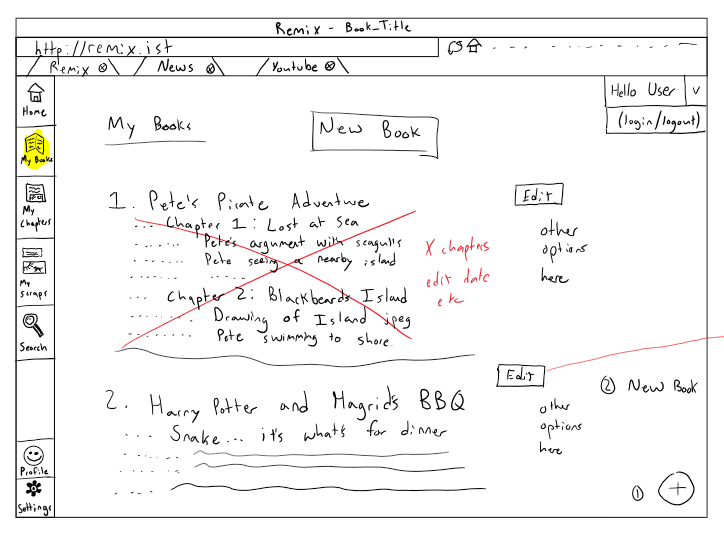
\includegraphics[width=12cm]{images/prototype}
	\caption{Here is one low fidelity prototype that was shown to our client. Dr. Jensen suggested 
		removing the preview of chapters and scraps to make the interface a little more simple.}
\end{figure}

\begin{figure}[ht!]
	\centering
	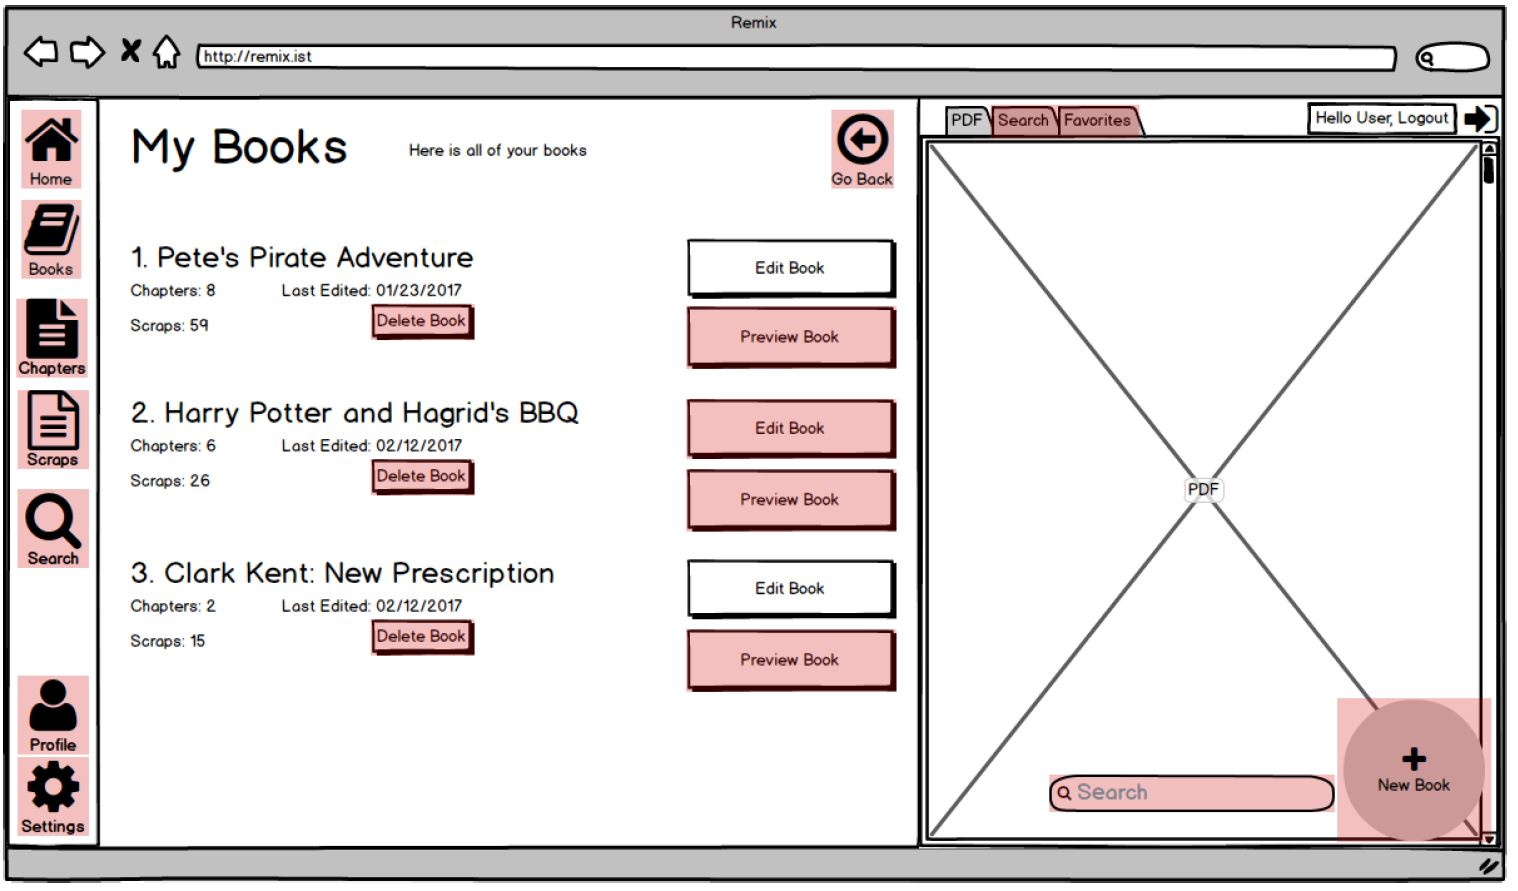
\includegraphics[width=12cm]{images/balsamiq}
	\caption{Here is one medium fidelity prototype, created in balsamiq, that allowed for users to provide feedback about the basic ideas of placement without worrying about finalized plans.}
\end{figure}

\begin{figure}[ht!]
	\centering
	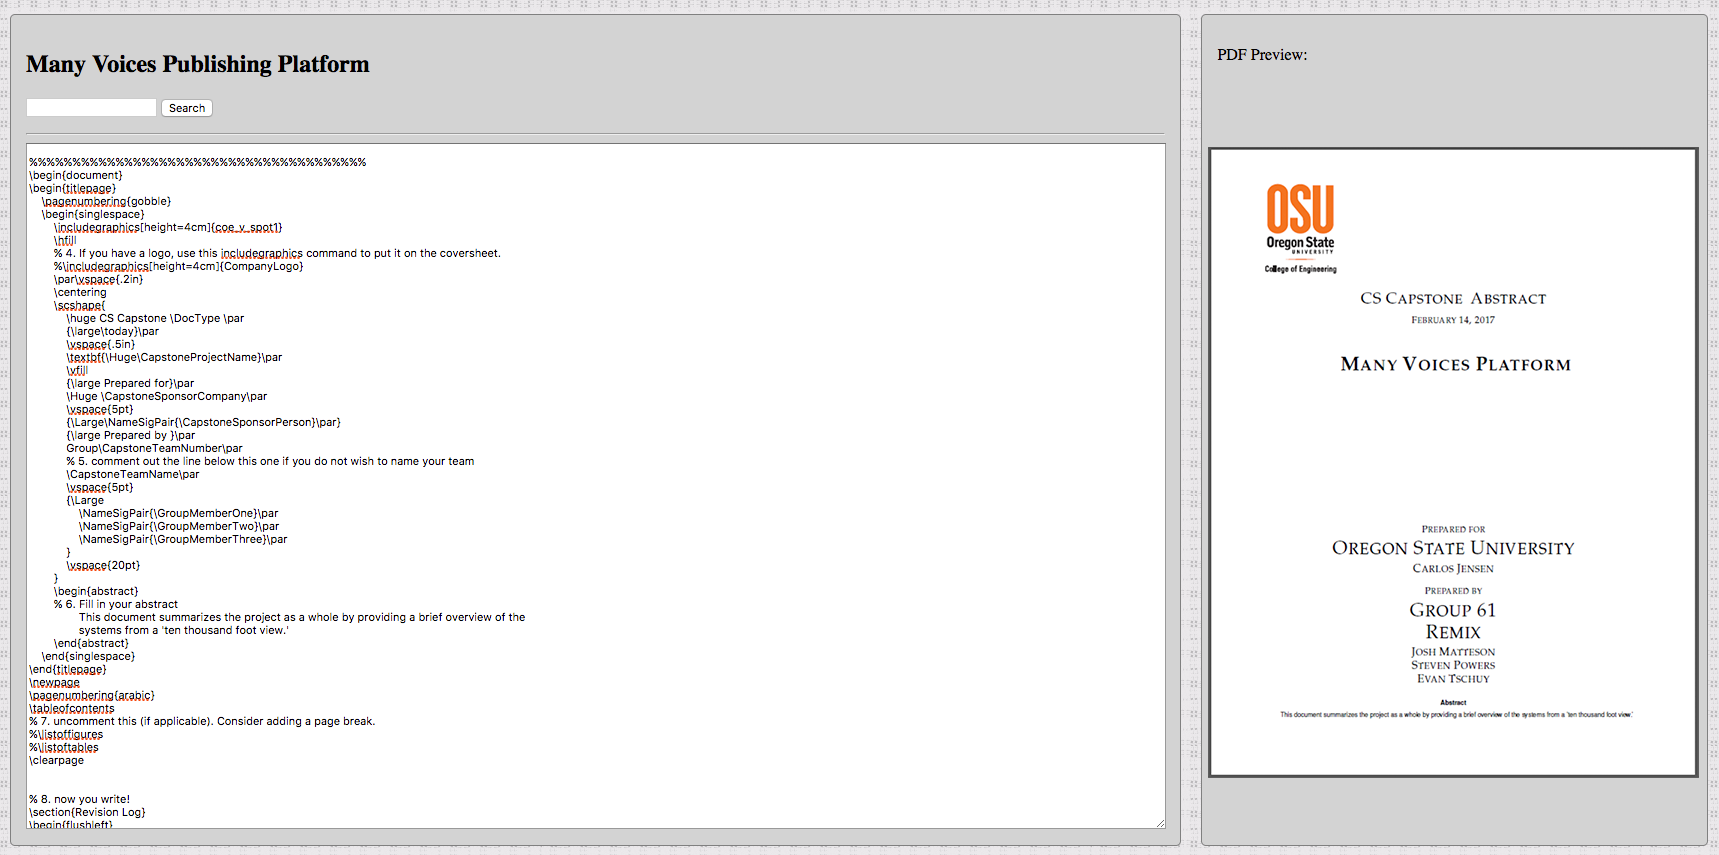
\includegraphics[width=12cm]{images/pdfpreview}
	\caption{Here is one high fidelity prototype. This was created using basic web HTML and our Aurelia framework and the use of a hard coded PDF to display a document. This was used as a learning exercise.}
\end{figure}

\begin{figure}[ht!]
	\centering
	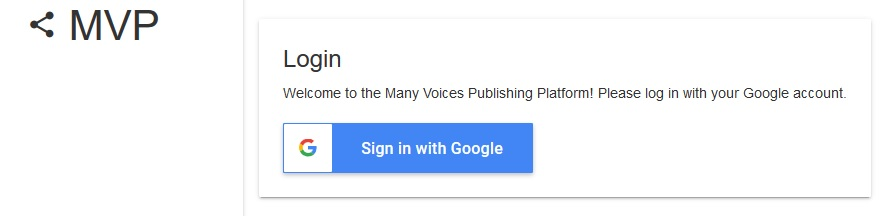
\includegraphics[width=12cm]{images/login_page}
	\caption{Here is the final product login page, which uses Google OAuth to abstract our need for security.}
\end{figure}

\begin{figure}[ht!]
	\centering
	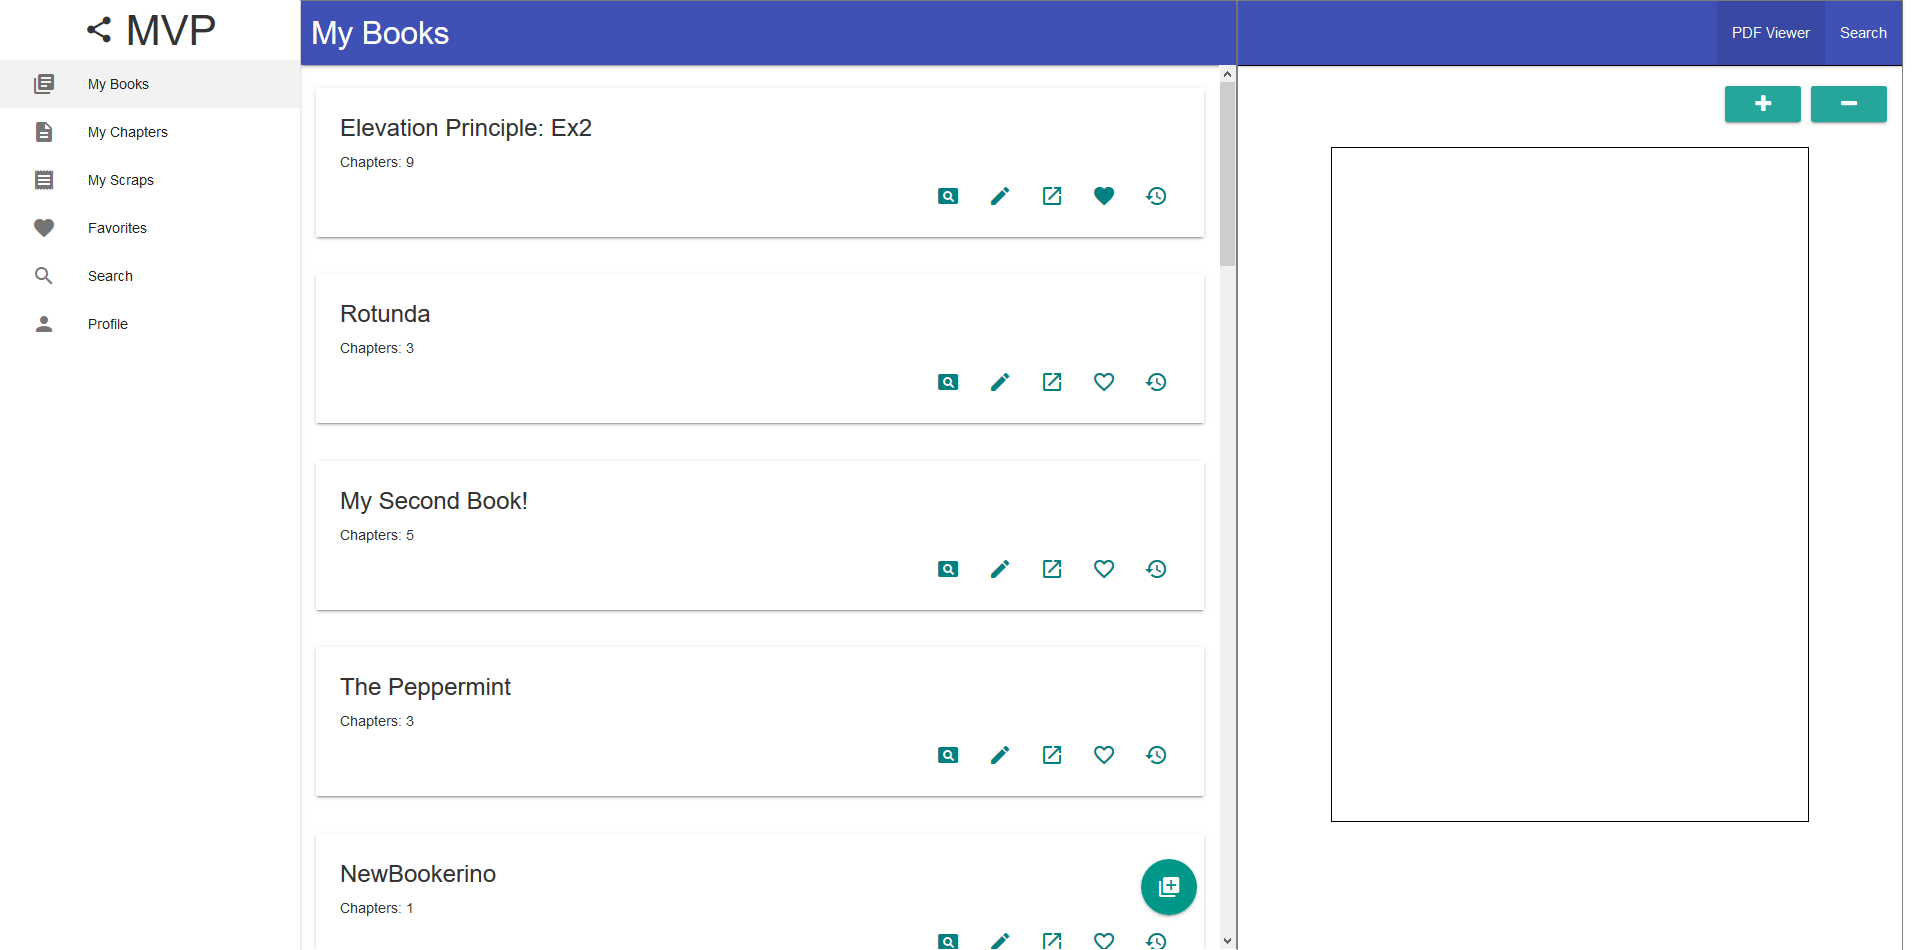
\includegraphics[width=12cm]{images/mybooks}
	\caption{Here is the final product my books page, showing sample textbook data.}
\end{figure}

\begin{figure}[ht!]
	\centering
	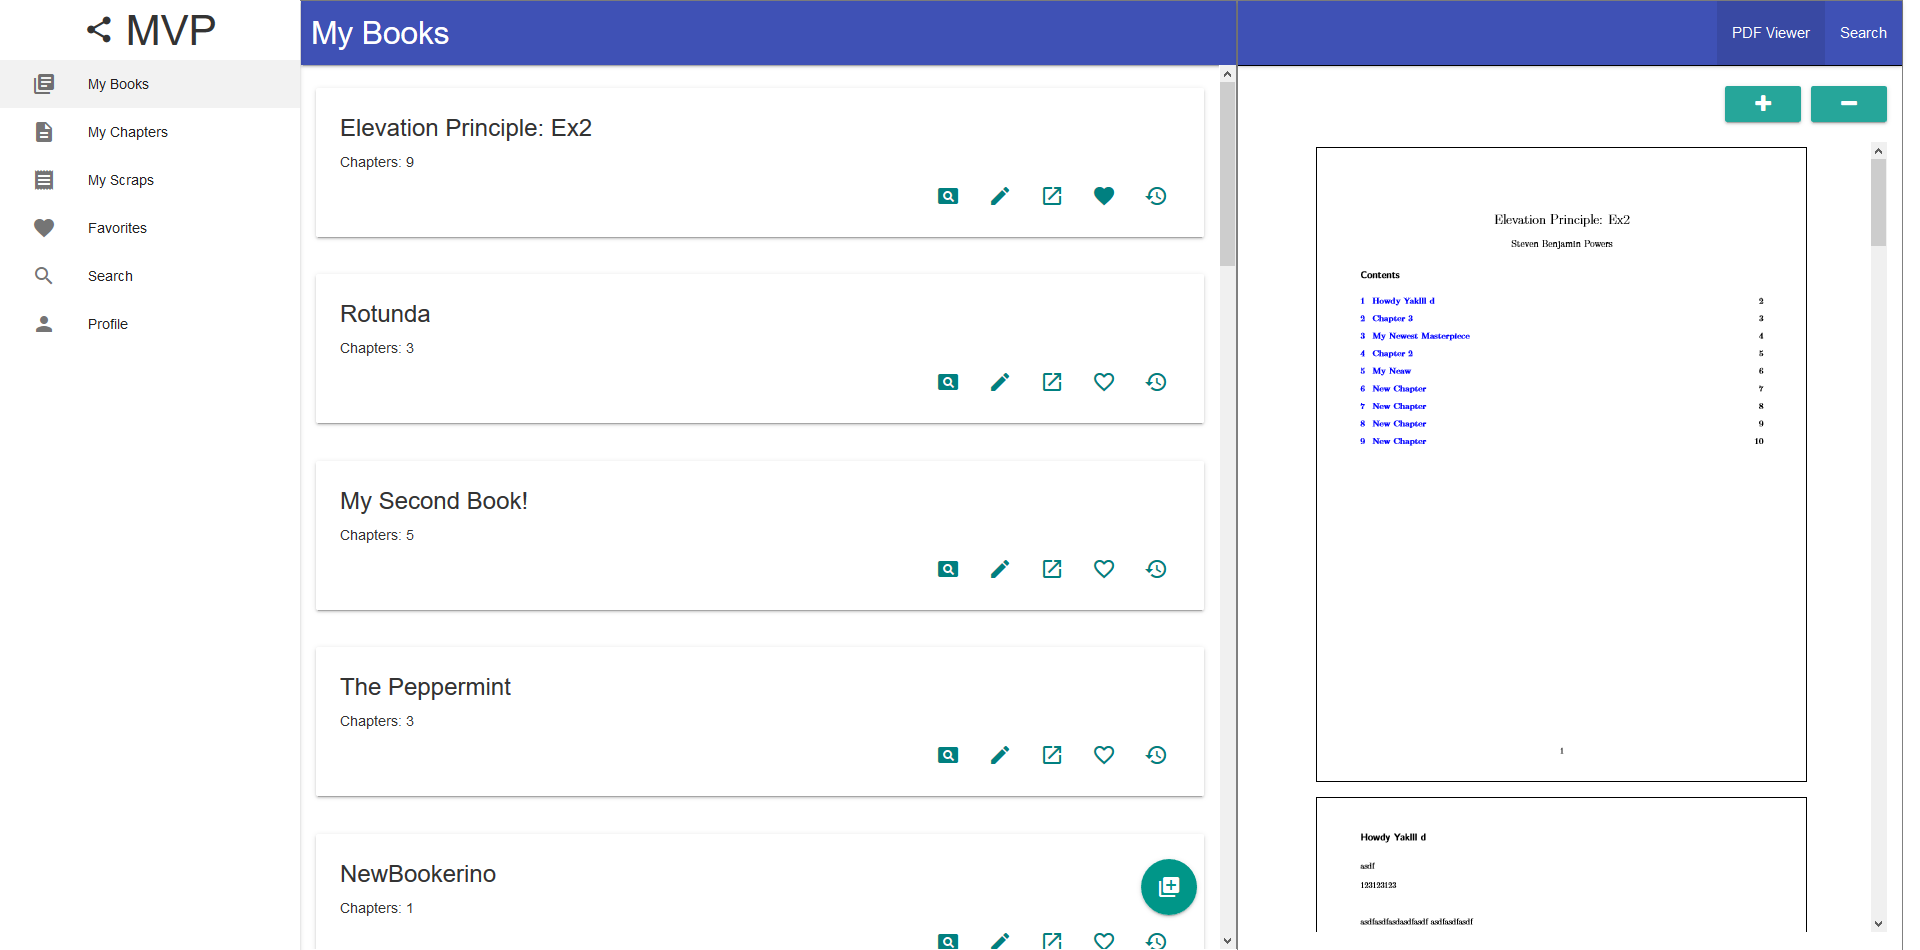
\includegraphics[width=12cm]{images/mybooks_preview}
	\caption{Here is the final product my books page, previewing a textbook.}
\end{figure}

\begin{figure}[ht!]
	\centering
	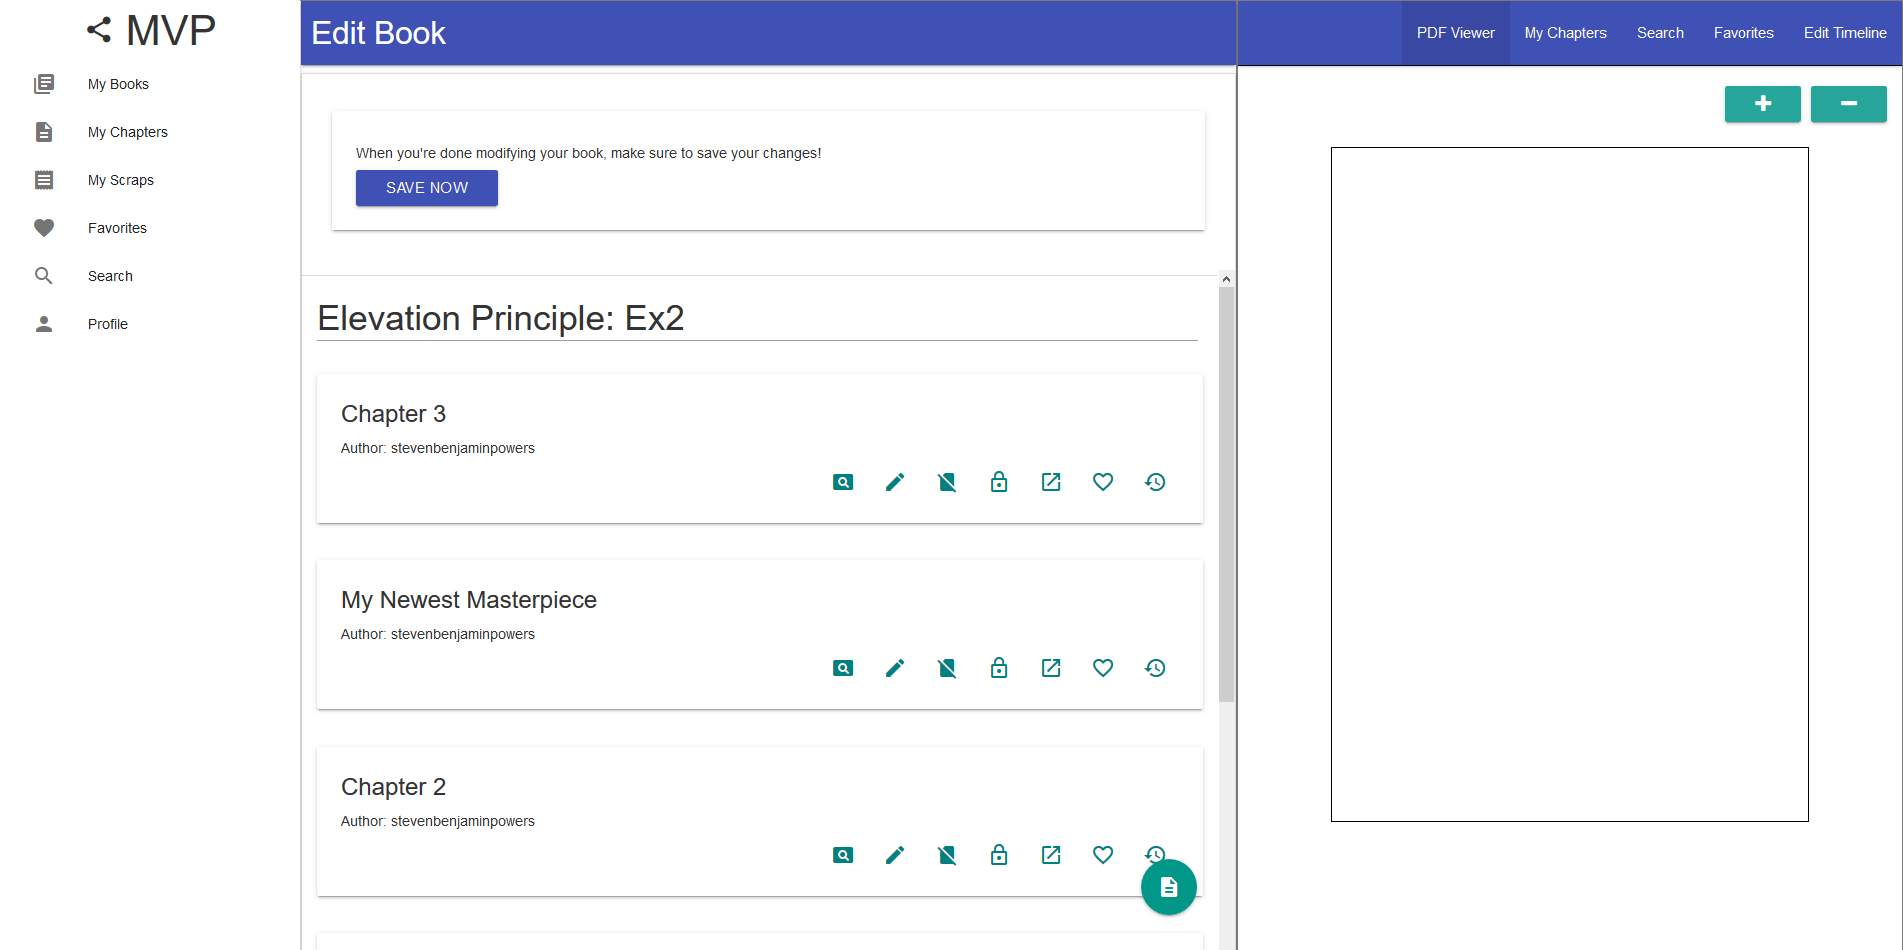
\includegraphics[width=12cm]{images/editbook}
	\caption{Here is the final product edit books page, allowing the user to edit chapters within a book.}
\end{figure}

\begin{figure}[ht!]
	\centering
	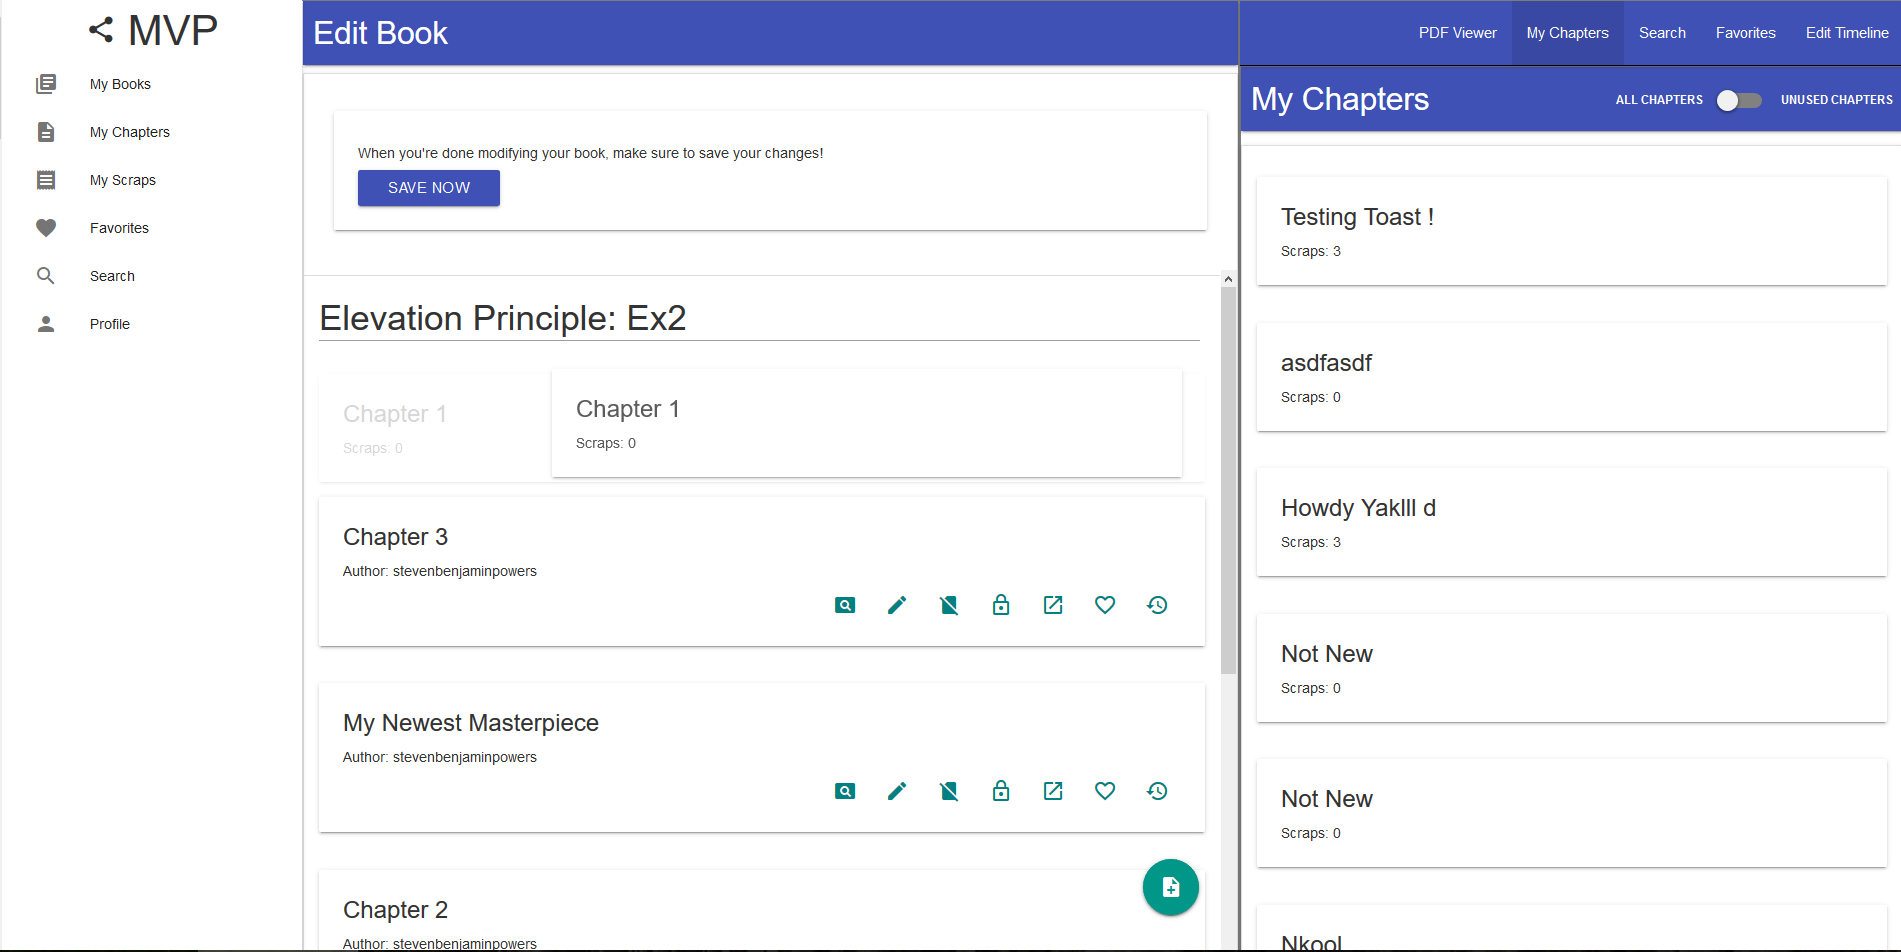
\includegraphics[width=12cm]{images/editbook_drag}
	\caption{Here is the final product edit books page, showing the use of drag and drop from a user's chapters.}
\end{figure}

\begin{figure}[ht!]
	\centering
	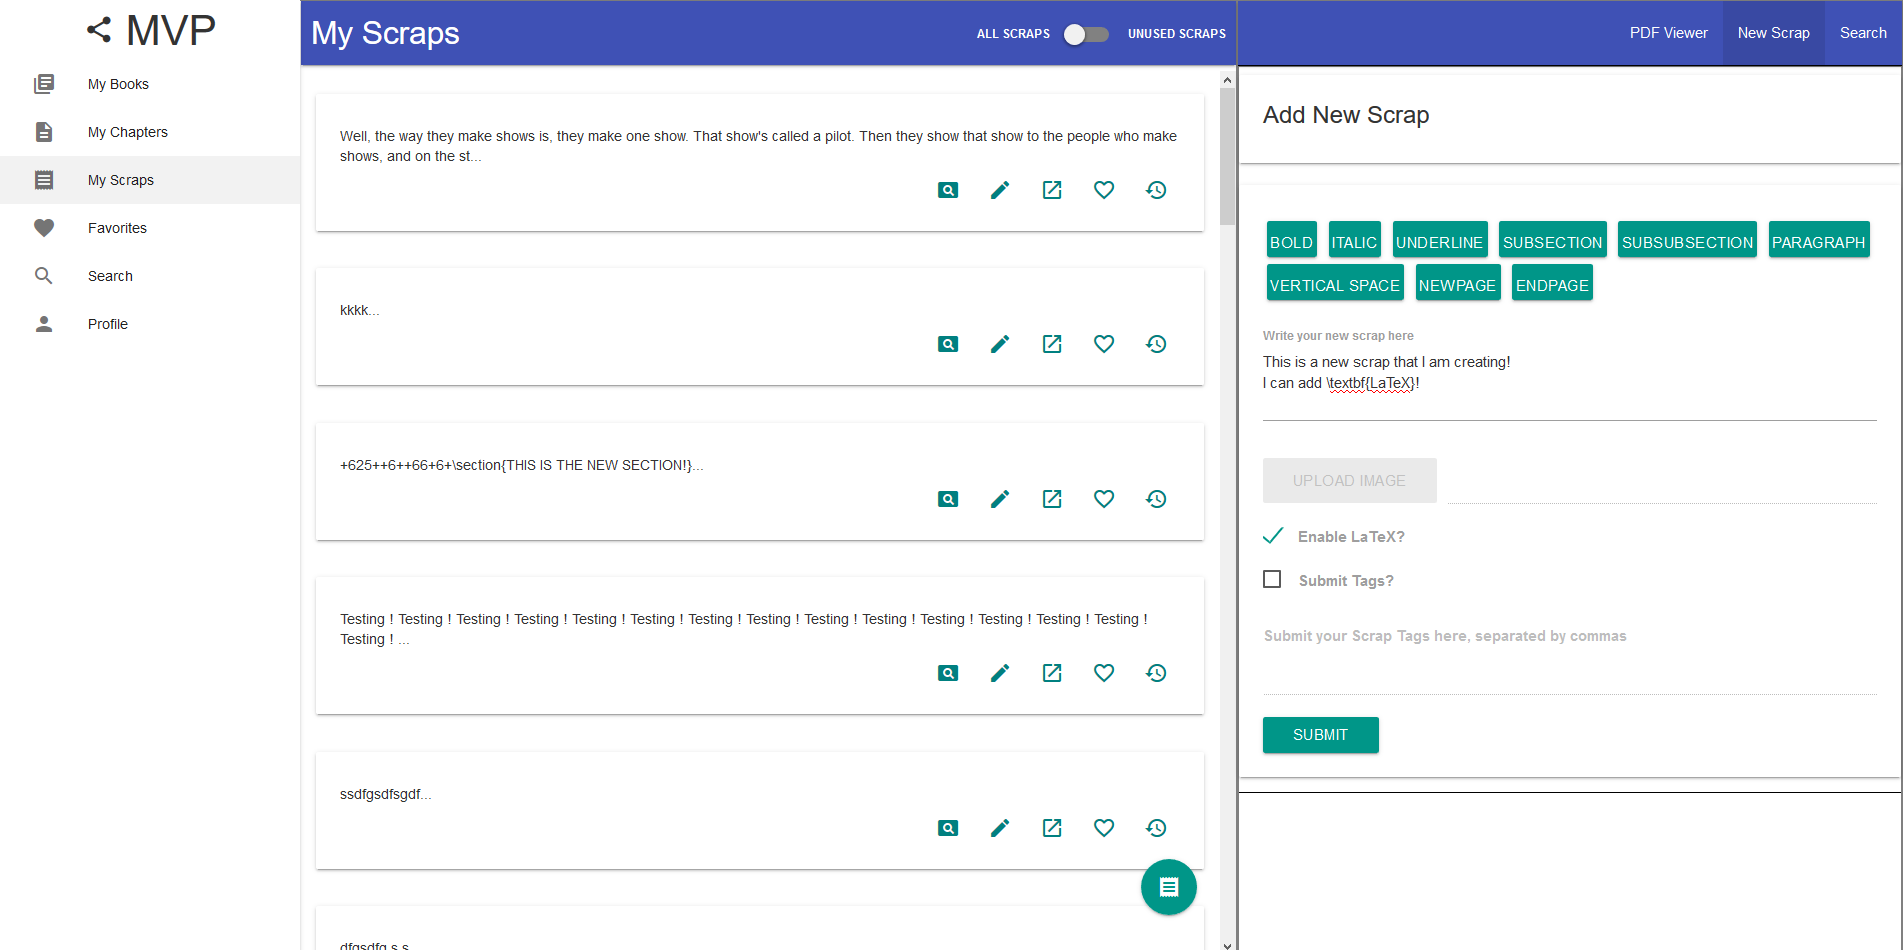
\includegraphics[width=12cm]{images/newscrap}
	\caption{Here is the final product new scrap page, showing how easy it is for a user to create a new scrap and even enable more advanced features by using LaTeX..}
\end{figure}

\clearpage
\newpage
\section{Conclusion}
\noindent The Many Voices Publishing Platform has been a great project to work on, bringing each team member outside their comfort zone. Our project has made enormous progress in the last few months that have enabled the platform to arrive on schedule for the Capstone Expo event. The team is proud of the product they have created, especially after the long and sometimes arduous journey from beginning to end.



\end{document}
